\section{Methodology}

\subsection{Datasets}
To train both the fine-tuned approach and the adapter-based approach datasets are necessary.
For the task of text simplification this is parallel data, meaning a pair of a complex text and it's simplified counterpart.
Table \ref{table:datasets} offers an overview of datasets that come into question as training data.

\textbf{Newsela} consist of mostly English news articles in different levels of simplification.
It contains the complex text and up to five simplified readability levels cultivated by professional authors~\cite{Xu2015}.
\citet{Jiang2020} manually labeled sentence alignments in the Newsela dataset ("Newsela Manual") to the train a neural CRF
sentence alignment method. This model is then used to get complex and simple sentence pairs from the entire corpus of
parallel documents ("Newsela Auto").
Since the auto dataset is considerably larger this will be used for creating a baseline.

\textbf{Klexikon} is a dataset for joint summarization and simplification and is created with semi-automated alignments between the German
Wikipedia and a German encyclopedia for children. Since it's aligned between Wikipedia articles and entries of an encyclopedia, it is document based~\cite{Aumiller2022}.

\textbf{GEOLino} contains data from a German general-interest children magazine, called GEOLino. ~\citet{Mallinson2020} used it in their research as a test set,
which was created manually by a trained linguist from 20 extracted articles.

\textbf{TextComplexity} is a dataset consisting of sentences from Wikipedia, which were assessed as complex by German learners in level
A and B. A native German speaker manually simplified 250 of these sentences and the simplifications were rated by the language learners
regarding their simplicity~\cite{Mallinson2020}.

\textbf{Cochrane} consists of text from the medical domain, extracted from the Cochrane Database of Systematic Reviews.
These reviews are documents containing a technical (complex) and a plain language summary (simple) version.
The simplified version is addressed to ``most readers without a university education'' and is written by review authors~\cite{Devaraj2021}.
Both document versions are not aligned, however ~\citet{Devaraj2021} treat the paragraphs \emph{results}, \emph{discussion} and \emph{conclusion}
as parallel data.
Also, every review is translated into multiple other languages.

\begin{table}[h!]
    \centering
    \begin{tabular}{ |p{3cm}|p{2.5cm}|p{2.5cm}|p{2.5cm}|p{2.5cm}| }
        \hline
        \multicolumn{5}{|c|}{Datasets} \\
        \hline
        Dataset & Granularity & Language & \# Documents & \# Sent./Para. Pairs \\
        \hline
        Newsela Auto~\cite{Xu2015} & Doc/Sent & en/es & 1882 & 666,645 \\
        Klexikon~\cite{Aumiller2022} & Doc & de & 2898 & - \\
        GEOLino~\cite{Mallinson2020} & Sent & de & - & 663 \\
        TextComplexity~\cite{Mallinson2020} & Sent & de & - & 250 \\
        Cochrane~\cite{Devaraj2021} & Paragraph & multi & 8944 & - \\
        \hline
    \end{tabular}
    \caption{Parallel Corpora for Text Simplification\\
        Corpora differ in their level of detail (Granularity; available on sentence, paragraph or document level)
    }
    \label{table:datasets}
\end{table}


\subsection{Baseline Text Simplification models using English and German parallel data}
To compare the performance of adapters in text simplification a meaningful baseline is necessary.
Therefore, reference models should be trained by fine-tuning a pretrained model.
As a pretrained model one option would be BART, since it's a sequence-to-sequence model
built upon a bidirectional encoder and an autoregressive decoder~\cite{Lewis2019}.
This makes it effective model when fine-tuned for text generation tasks~\cite{Lewis2019}.
For creating the baseline labeled data in the target language is necessary, meaning this includes a German dataset to compare against
an adapter-based model which hasn't seen any German data.
The fine-tuning process should be done using each of the datasets mentioned above,
resulting in an English and a German fine-tuned TS model.
Figure \ref{fig:finetuning} gives an overview of the fine-tuning of the language model.
Fine-tuning will be done using the Huggingface library, since it's offering an end-to-end
integration of loading the pretrained model, training it, evaluating it and deploying the model~\cite{Huggingface2023}.
Each of the fine-tuned models is then evaluated against a test set to see how this
baseline performs.

\begin{figure}
    \centering
    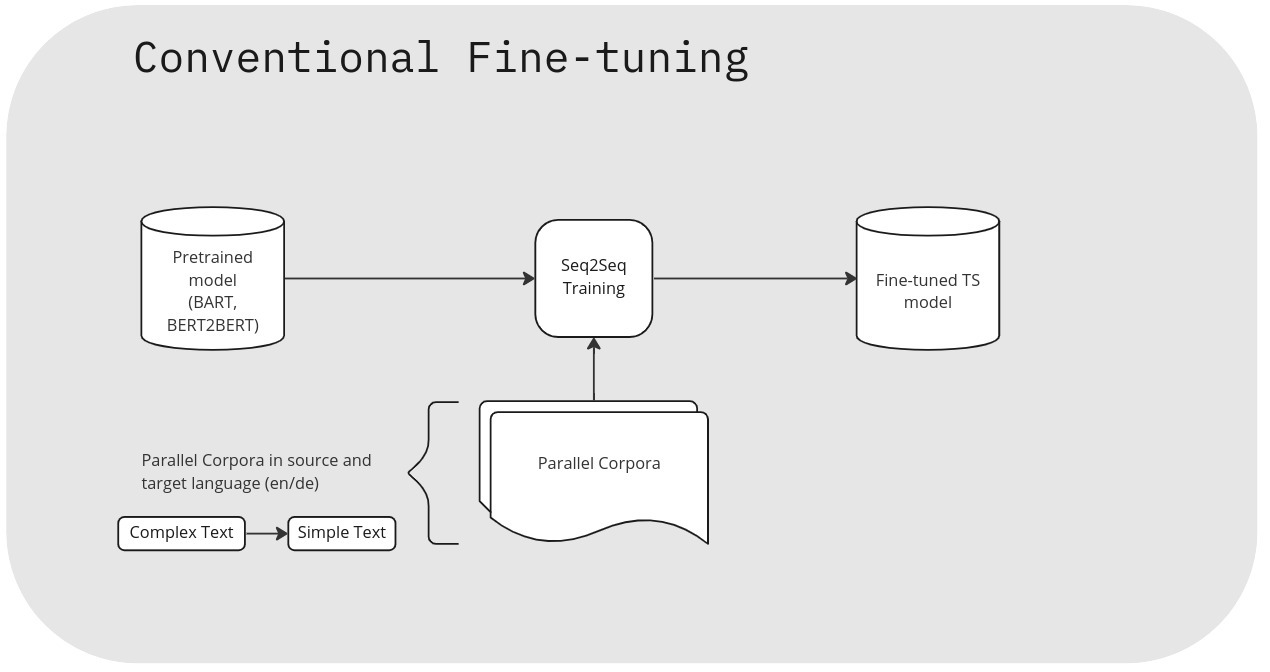
\includegraphics[width=\textwidth]{./figures/finetuning.jpg}
    \caption{Fine-tuning a pretrained model using parallel copora}
    \Description[Fine-tuning a pretrained model]{Fine-tuning a pretrained model}
    \label{fig:finetuning}
\end{figure}

\subsection{Adapters for Text Simplification without German data}
After fully fine-tuning TS models with a pre-trained model as a baseline,
Adapters for the desired tasks should be trained.
To have a fair comparison between the baseline and the adapters the same pretrained model
should be utilized, meaning the adapters will likely be trained on BART.
Training the adapters could be done using Adapterhub, which is built on top of Huggingface~\cite{Pfeiffer2023}.
To make use of the composable nature of adapters first the adapter for the TS task should be trained
on an English dataset, namely Newsela Auto.
With a pretrained language adapter for German from the Adapterhub the previously trained TS task adapter should be combined
to then compare the results to a fully fine-tuned model.
In this setup no German parallel data is involved during training the text simplification model. This condition will be used to then see how
adapters perform compared to a fine-tuned model, which was trained using parallel data in the target language.
Figure \ref{fig:adapters} shows the overall process of integrating a task adapter into a pretrained model, training it and using it combined
with a language adapter during inference. Training the adapter is done using data only in a source language e.g., English in a 
zero-shot setting and parallel data using a small amount of data in the target language e.g., German.

\begin{figure}
    \centering
    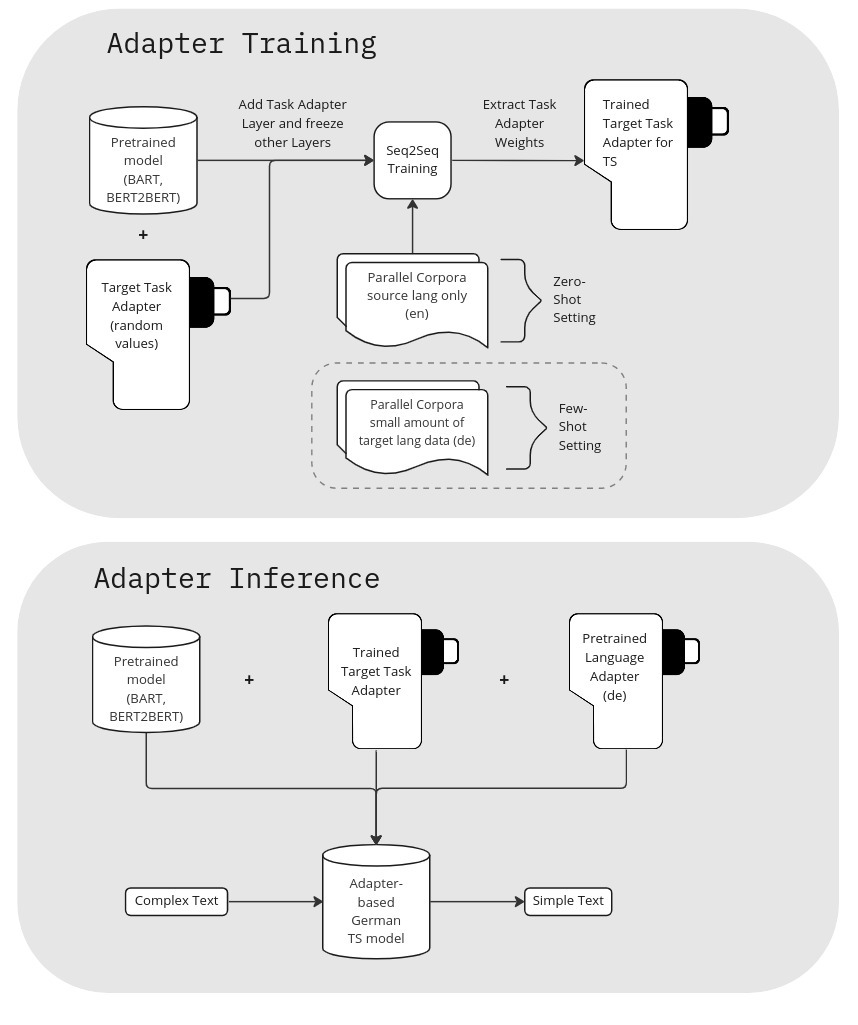
\includegraphics[width=\textwidth]{./figures/adapter-setup.jpg}
    \caption{Training and using a Task Adapter for Text Simplification. First the task adapter is initialized and inserted
    into the pretrained model. The weights of the pretrained model are then frozen and the adapter weights are trained
    using parallel corpora in English (in a zero-shot setting) and some German samples (in a few-shot setting).
    During inference the extracted adapter is then used with a pretrained language adapter.}
    \Description[Fine-tuning a pretrained model]{Fine-tuning a pretrained model}
    \label{fig:adapters}
\end{figure}

\subsection{Evaluation}
Both approaches, the fine-tuned and the adapter based models should be evaluated
using common evaluation metrics for text simplification.
Automatic metrics should be used to for determine the similarity and the simplicity of the text.
As a measurement for the similarity of the produced output and the test set, BLEU, TER and FKGL should be used~\cite{AlvaManchego2020}.
Evaluation of simplicity of the produced text should be done by SARI~\cite{AlvaManchego2020}.
Automatic metrics are easy and cheaper to calculate, however it is questionable if they work properly for document level
simplifications. Therefore, when doing document level simplifications human evaluation might be a better approach.
Metrics for computational efficiency e.g., the number of parameters of a model, the computational time and flops during
training and inference should be measured.
To answer research question \ref{rq:1} and \ref{rq:2.1} automatic metrics should be used to evaluate. Research question \ref{rq:2.2} can be answered
using metrics for computational efficiency. For research question \ref{rq:2.3} automatic metrics can be used, however it is unclear, if 
sentence/paragraph level models are comparable with document level models using these metrics. Therefor, a human evaluation might be better fitting.